\PassOptionsToPackage{unicode=true}{hyperref} % options for packages loaded elsewhere
\PassOptionsToPackage{hyphens}{url}
%
\documentclass[]{article}
\usepackage{lmodern}
\usepackage{amssymb,amsmath}
\usepackage{ifxetex,ifluatex}
\usepackage{fixltx2e} % provides \textsubscript
\ifnum 0\ifxetex 1\fi\ifluatex 1\fi=0 % if pdftex
  \usepackage[T1]{fontenc}
  \usepackage[utf8]{inputenc}
  \usepackage{textcomp} % provides euro and other symbols
\else % if luatex or xelatex
  \usepackage{unicode-math}
  \defaultfontfeatures{Ligatures=TeX,Scale=MatchLowercase}
\fi
% use upquote if available, for straight quotes in verbatim environments
\IfFileExists{upquote.sty}{\usepackage{upquote}}{}
% use microtype if available
\IfFileExists{microtype.sty}{%
\usepackage[]{microtype}
\UseMicrotypeSet[protrusion]{basicmath} % disable protrusion for tt fonts
}{}
\IfFileExists{parskip.sty}{%
\usepackage{parskip}
}{% else
\setlength{\parindent}{0pt}
\setlength{\parskip}{6pt plus 2pt minus 1pt}
}
\usepackage{hyperref}
\hypersetup{
            pdftitle={knitr\_project},
            pdfauthor={iskren89},
            pdfborder={0 0 0},
            breaklinks=true}
\urlstyle{same}  % don't use monospace font for urls
\usepackage[margin=1in]{geometry}
\usepackage{color}
\usepackage{fancyvrb}
\newcommand{\VerbBar}{|}
\newcommand{\VERB}{\Verb[commandchars=\\\{\}]}
\DefineVerbatimEnvironment{Highlighting}{Verbatim}{commandchars=\\\{\}}
% Add ',fontsize=\small' for more characters per line
\usepackage{framed}
\definecolor{shadecolor}{RGB}{248,248,248}
\newenvironment{Shaded}{\begin{snugshade}}{\end{snugshade}}
\newcommand{\AlertTok}[1]{\textcolor[rgb]{0.94,0.16,0.16}{#1}}
\newcommand{\AnnotationTok}[1]{\textcolor[rgb]{0.56,0.35,0.01}{\textbf{\textit{#1}}}}
\newcommand{\AttributeTok}[1]{\textcolor[rgb]{0.77,0.63,0.00}{#1}}
\newcommand{\BaseNTok}[1]{\textcolor[rgb]{0.00,0.00,0.81}{#1}}
\newcommand{\BuiltInTok}[1]{#1}
\newcommand{\CharTok}[1]{\textcolor[rgb]{0.31,0.60,0.02}{#1}}
\newcommand{\CommentTok}[1]{\textcolor[rgb]{0.56,0.35,0.01}{\textit{#1}}}
\newcommand{\CommentVarTok}[1]{\textcolor[rgb]{0.56,0.35,0.01}{\textbf{\textit{#1}}}}
\newcommand{\ConstantTok}[1]{\textcolor[rgb]{0.00,0.00,0.00}{#1}}
\newcommand{\ControlFlowTok}[1]{\textcolor[rgb]{0.13,0.29,0.53}{\textbf{#1}}}
\newcommand{\DataTypeTok}[1]{\textcolor[rgb]{0.13,0.29,0.53}{#1}}
\newcommand{\DecValTok}[1]{\textcolor[rgb]{0.00,0.00,0.81}{#1}}
\newcommand{\DocumentationTok}[1]{\textcolor[rgb]{0.56,0.35,0.01}{\textbf{\textit{#1}}}}
\newcommand{\ErrorTok}[1]{\textcolor[rgb]{0.64,0.00,0.00}{\textbf{#1}}}
\newcommand{\ExtensionTok}[1]{#1}
\newcommand{\FloatTok}[1]{\textcolor[rgb]{0.00,0.00,0.81}{#1}}
\newcommand{\FunctionTok}[1]{\textcolor[rgb]{0.00,0.00,0.00}{#1}}
\newcommand{\ImportTok}[1]{#1}
\newcommand{\InformationTok}[1]{\textcolor[rgb]{0.56,0.35,0.01}{\textbf{\textit{#1}}}}
\newcommand{\KeywordTok}[1]{\textcolor[rgb]{0.13,0.29,0.53}{\textbf{#1}}}
\newcommand{\NormalTok}[1]{#1}
\newcommand{\OperatorTok}[1]{\textcolor[rgb]{0.81,0.36,0.00}{\textbf{#1}}}
\newcommand{\OtherTok}[1]{\textcolor[rgb]{0.56,0.35,0.01}{#1}}
\newcommand{\PreprocessorTok}[1]{\textcolor[rgb]{0.56,0.35,0.01}{\textit{#1}}}
\newcommand{\RegionMarkerTok}[1]{#1}
\newcommand{\SpecialCharTok}[1]{\textcolor[rgb]{0.00,0.00,0.00}{#1}}
\newcommand{\SpecialStringTok}[1]{\textcolor[rgb]{0.31,0.60,0.02}{#1}}
\newcommand{\StringTok}[1]{\textcolor[rgb]{0.31,0.60,0.02}{#1}}
\newcommand{\VariableTok}[1]{\textcolor[rgb]{0.00,0.00,0.00}{#1}}
\newcommand{\VerbatimStringTok}[1]{\textcolor[rgb]{0.31,0.60,0.02}{#1}}
\newcommand{\WarningTok}[1]{\textcolor[rgb]{0.56,0.35,0.01}{\textbf{\textit{#1}}}}
\usepackage{graphicx,grffile}
\makeatletter
\def\maxwidth{\ifdim\Gin@nat@width>\linewidth\linewidth\else\Gin@nat@width\fi}
\def\maxheight{\ifdim\Gin@nat@height>\textheight\textheight\else\Gin@nat@height\fi}
\makeatother
% Scale images if necessary, so that they will not overflow the page
% margins by default, and it is still possible to overwrite the defaults
% using explicit options in \includegraphics[width, height, ...]{}
\setkeys{Gin}{width=\maxwidth,height=\maxheight,keepaspectratio}
\setlength{\emergencystretch}{3em}  % prevent overfull lines
\providecommand{\tightlist}{%
  \setlength{\itemsep}{0pt}\setlength{\parskip}{0pt}}
\setcounter{secnumdepth}{0}
% Redefines (sub)paragraphs to behave more like sections
\ifx\paragraph\undefined\else
\let\oldparagraph\paragraph
\renewcommand{\paragraph}[1]{\oldparagraph{#1}\mbox{}}
\fi
\ifx\subparagraph\undefined\else
\let\oldsubparagraph\subparagraph
\renewcommand{\subparagraph}[1]{\oldsubparagraph{#1}\mbox{}}
\fi

% set default figure placement to htbp
\makeatletter
\def\fps@figure{htbp}
\makeatother


\title{knitr\_project}
\author{iskren89}
\date{7/5/2020}

\begin{document}
\maketitle

\hypertarget{reproducible-research-project}{%
\section{Reproducible research
project}\label{reproducible-research-project}}

\textbf{1. Here we are loading and preprocessing the data}

\begin{Shaded}
\begin{Highlighting}[]
\KeywordTok{library}\NormalTok{(dplyr)}
\end{Highlighting}
\end{Shaded}

\begin{verbatim}
## 
## Attaching package: 'dplyr'
\end{verbatim}

\begin{verbatim}
## The following objects are masked from 'package:stats':
## 
##     filter, lag
\end{verbatim}

\begin{verbatim}
## The following objects are masked from 'package:base':
## 
##     intersect, setdiff, setequal, union
\end{verbatim}

\begin{Shaded}
\begin{Highlighting}[]
\NormalTok{temp <-}\StringTok{ }\KeywordTok{tempfile}\NormalTok{()}
\KeywordTok{download.file}\NormalTok{(}\StringTok{"https://d396qusza40orc.cloudfront.net/repdata%2Fdata%2Factivity.zip"}\NormalTok{,temp)}
\NormalTok{my_file <-}\StringTok{ }\KeywordTok{unz}\NormalTok{(temp, }\StringTok{"activity.csv"}\NormalTok{)}
\NormalTok{dat <-}\StringTok{ }\KeywordTok{read.csv}\NormalTok{(my_file)}
\NormalTok{dat[,}\DecValTok{3}\NormalTok{]<-}\KeywordTok{factor}\NormalTok{(dat[,}\DecValTok{3}\NormalTok{])}
\NormalTok{missing<-}\KeywordTok{sum}\NormalTok{(}\KeywordTok{is.na}\NormalTok{(dat}\OperatorTok{$}\NormalTok{steps))}
\KeywordTok{unlink}\NormalTok{(temp)}
\end{Highlighting}
\end{Shaded}

\textbf{2. Here we plot the total number of steps taken each day}

\begin{Shaded}
\begin{Highlighting}[]
\NormalTok{by_date<-}\KeywordTok{group_by}\NormalTok{(dat,date)}
\NormalTok{total_date<-}\KeywordTok{summarise}\NormalTok{(by_date,}\DataTypeTok{sum=}\KeywordTok{sum}\NormalTok{(steps),}\DataTypeTok{.groups =} \StringTok{'keep'}\NormalTok{)}
\KeywordTok{with}\NormalTok{(total_date, }\KeywordTok{hist}\NormalTok{(sum,}\DataTypeTok{main=}\StringTok{"Total number of steps"}\NormalTok{,}\DataTypeTok{xlab=}\StringTok{""}\NormalTok{))}
\end{Highlighting}
\end{Shaded}

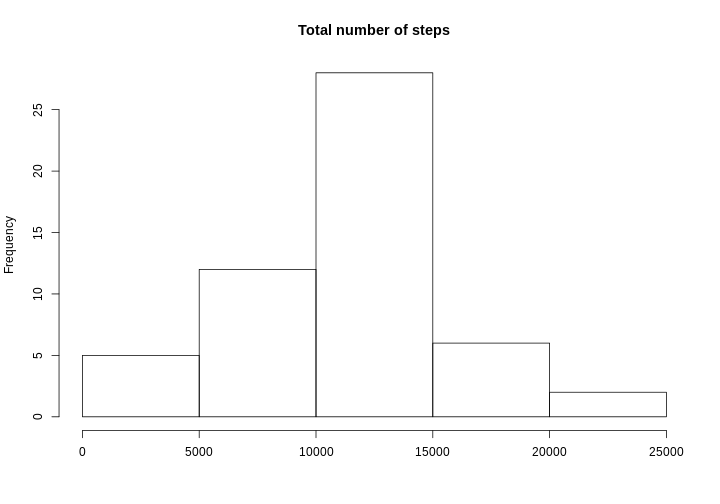
\includegraphics{my_project_files/figure-latex/unnamed-chunk-2-1.pdf}
\textbf{3. Here we calculate the mean and median number of steps taken
each day}

\begin{Shaded}
\begin{Highlighting}[]
\KeywordTok{summary}\NormalTok{(total_date)}
\end{Highlighting}
\end{Shaded}

\begin{verbatim}
##          date         sum       
##  2012-10-01: 1   Min.   :   41  
##  2012-10-02: 1   1st Qu.: 8841  
##  2012-10-03: 1   Median :10765  
##  2012-10-04: 1   Mean   :10766  
##  2012-10-05: 1   3rd Qu.:13294  
##  2012-10-06: 1   Max.   :21194  
##  (Other)   :55   NA's   :8
\end{verbatim}

\textbf{4. Here we show the time series plot of the average number of
steps taken}

\begin{Shaded}
\begin{Highlighting}[]
\NormalTok{by_interval<-}\KeywordTok{group_by}\NormalTok{(dat,interval)}
\NormalTok{mean_interval<-}\KeywordTok{summarise}\NormalTok{(by_interval,}\DataTypeTok{mean=}\KeywordTok{mean}\NormalTok{(steps,}\DataTypeTok{na.rm=}\OtherTok{TRUE}\NormalTok{),}\DataTypeTok{.groups =} \StringTok{'keep'}\NormalTok{)}
\KeywordTok{with}\NormalTok{(mean_interval, }\KeywordTok{plot}\NormalTok{(interval,mean,}\DataTypeTok{type =} \StringTok{"l"}\NormalTok{,}\DataTypeTok{main=}\StringTok{"Average number of steps"}\NormalTok{,}\DataTypeTok{ylab=}\StringTok{"steps by 5-minute interval"}\NormalTok{))}
\end{Highlighting}
\end{Shaded}

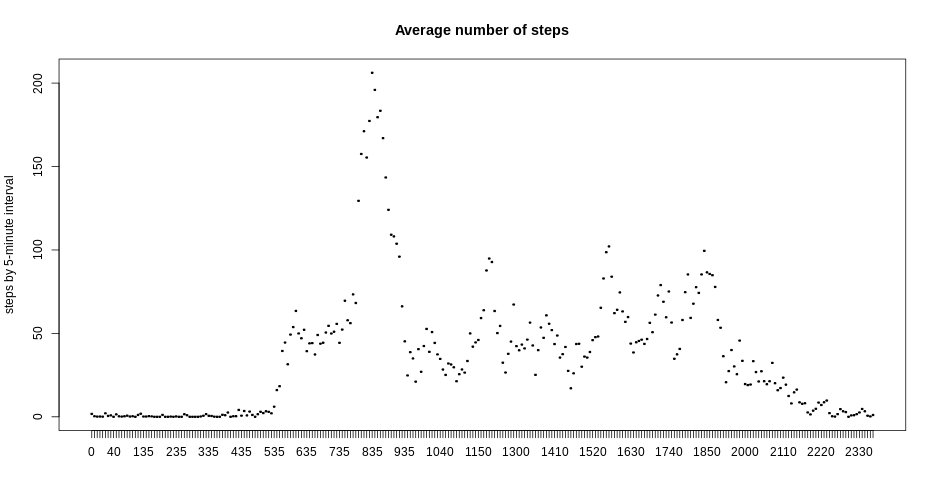
\includegraphics{my_project_files/figure-latex/unnamed-chunk-4-1.pdf}
\textbf{5. The 5-minute interval that, on average, contains the maximum
number of step is:}

\begin{Shaded}
\begin{Highlighting}[]
\NormalTok{mean_interval[}\KeywordTok{which.max}\NormalTok{(mean_interval}\OperatorTok{$}\NormalTok{mean),]}
\end{Highlighting}
\end{Shaded}

\begin{verbatim}
## # A tibble: 1 x 2
## # Groups:   interval [1]
##   interval  mean
##   <fct>    <dbl>
## 1 835       206.
\end{verbatim}

\textbf{6. Here we describe and show a strategy for imputing missing
data}\\
There are 2304 missing values in the original dataset - there are 8 days
for which there is no data.\\
We will impute the missing data by using the mean for that 5-minute
interval.

\begin{Shaded}
\begin{Highlighting}[]
\NormalTok{impute.mean <-}\StringTok{ }\ControlFlowTok{function}\NormalTok{(x) }\KeywordTok{replace}\NormalTok{(x, }\KeywordTok{is.na}\NormalTok{(x), }\KeywordTok{mean}\NormalTok{(x, }\DataTypeTok{na.rm =} \OtherTok{TRUE}\NormalTok{))}
\NormalTok{imputed<-}\KeywordTok{mutate}\NormalTok{(by_interval,}\DataTypeTok{steps =} \KeywordTok{impute.mean}\NormalTok{(steps))}
\end{Highlighting}
\end{Shaded}

\textbf{7. Here we show a histogram of the total number of steps taken
each day after missing values are imputed}

\begin{Shaded}
\begin{Highlighting}[]
\NormalTok{imputed_by_date<-}\KeywordTok{group_by}\NormalTok{(imputed,date)}
\NormalTok{imputed_total_date<-}\KeywordTok{summarise}\NormalTok{(imputed_by_date,}\DataTypeTok{sum=}\KeywordTok{sum}\NormalTok{(steps),}\DataTypeTok{.groups =} \StringTok{'keep'}\NormalTok{)}
\KeywordTok{with}\NormalTok{(imputed_total_date, }\KeywordTok{hist}\NormalTok{(sum,}\DataTypeTok{main=}\StringTok{"Total number of steps"}\NormalTok{,}\DataTypeTok{xlab=}\StringTok{""}\NormalTok{))}
\end{Highlighting}
\end{Shaded}

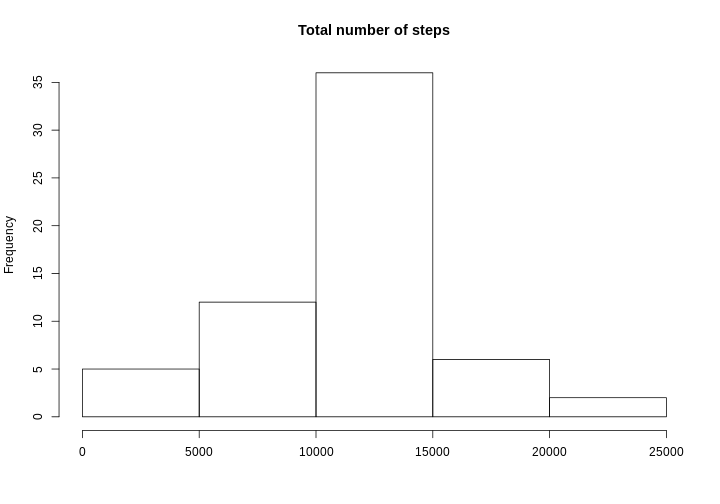
\includegraphics{my_project_files/figure-latex/unnamed-chunk-7-1.pdf} We
see that the profile of the data does not change after we impute it.

\begin{Shaded}
\begin{Highlighting}[]
\KeywordTok{summary}\NormalTok{(imputed_total_date)}
\end{Highlighting}
\end{Shaded}

\begin{verbatim}
##          date         sum       
##  2012-10-01: 1   Min.   :   41  
##  2012-10-02: 1   1st Qu.: 9819  
##  2012-10-03: 1   Median :10766  
##  2012-10-04: 1   Mean   :10766  
##  2012-10-05: 1   3rd Qu.:12811  
##  2012-10-06: 1   Max.   :21194  
##  (Other)   :55
\end{verbatim}

\emph{Note that in the original calculation and histogram I do not
remove the 8 days for which we have no data.}\\
\emph{If you use na.rm=TRUE to remove the missing values, they are still
counted as 0 in any summary statistics.}\\
\emph{As a result the mean/median total number of steps per day will be
lower, because the 8 missing days are all taken as 0 in the numerator,
while the denominator is higher.}\\
\emph{I took this approach because I think it's unrealistic that no
steps were taken on those 8 days.}\\
\emph{Rather the more plausible explanation is that the person did not
wear his or hers activity tracker on that day. The effect of this can be
seen below.}

\emph{Missing data not removed from the original data set. Note that
there are 8 missing values and the minimum number of steps is 41:}

\begin{Shaded}
\begin{Highlighting}[]
\KeywordTok{summary}\NormalTok{(total_date)}
\end{Highlighting}
\end{Shaded}

\begin{verbatim}
##          date         sum       
##  2012-10-01: 1   Min.   :   41  
##  2012-10-02: 1   1st Qu.: 8841  
##  2012-10-03: 1   Median :10765  
##  2012-10-04: 1   Mean   :10766  
##  2012-10-05: 1   3rd Qu.:13294  
##  2012-10-06: 1   Max.   :21194  
##  (Other)   :55   NA's   :8
\end{verbatim}

\emph{Missing data removed from the original data set. Note that there
are no missing values and the minimum number of steps is 0:}

\begin{Shaded}
\begin{Highlighting}[]
\NormalTok{removed_total_date<-}\KeywordTok{summarise}\NormalTok{(by_date,}\DataTypeTok{sum=}\KeywordTok{sum}\NormalTok{(steps,}\DataTypeTok{na.rm=}\OtherTok{TRUE}\NormalTok{),}\DataTypeTok{.groups =} \StringTok{'keep'}\NormalTok{)}
\KeywordTok{summary}\NormalTok{(removed_total_date)}
\end{Highlighting}
\end{Shaded}

\begin{verbatim}
##          date         sum       
##  2012-10-01: 1   Min.   :    0  
##  2012-10-02: 1   1st Qu.: 6778  
##  2012-10-03: 1   Median :10395  
##  2012-10-04: 1   Mean   : 9354  
##  2012-10-05: 1   3rd Qu.:12811  
##  2012-10-06: 1   Max.   :21194  
##  (Other)   :55
\end{verbatim}

\textbf{8. Here we make a panel plot comparing the average number of
steps taken per 5-minute interval across weekdays and weekends}

\begin{Shaded}
\begin{Highlighting}[]
\NormalTok{imputed}\OperatorTok{$}\NormalTok{date<-}\KeywordTok{as.Date}\NormalTok{(imputed}\OperatorTok{$}\NormalTok{date)}
\NormalTok{imputed}\OperatorTok{$}\NormalTok{weekday<-}\KeywordTok{as.factor}\NormalTok{(}\KeywordTok{weekdays}\NormalTok{(imputed}\OperatorTok{$}\NormalTok{date))}
\NormalTok{weekend <-}\StringTok{ }\KeywordTok{c}\NormalTok{(}\StringTok{"Saturday"}\NormalTok{,}\StringTok{"Sunday"}\NormalTok{)}
\NormalTok{imputed}\OperatorTok{$}\NormalTok{weekend <-}\StringTok{ }\KeywordTok{as.factor}\NormalTok{(}\KeywordTok{ifelse}\NormalTok{(imputed}\OperatorTok{$}\NormalTok{weekday }\OperatorTok\StringTok{ }\NormalTok{weekend, }\StringTok{"weekend"}\NormalTok{,}\StringTok{"weekday"}\NormalTok{))}
\NormalTok{imputed_weekdays<-}\KeywordTok{filter}\NormalTok{(imputed,weekend}\OperatorTok{==}\StringTok{"weekday"}\NormalTok{)}
\NormalTok{imputed_weekends<-}\KeywordTok{filter}\NormalTok{(imputed,weekend}\OperatorTok{==}\StringTok{"weekend"}\NormalTok{)}
\NormalTok{weekdays_interval<-}\KeywordTok{group_by}\NormalTok{(imputed_weekdays,interval)}
\NormalTok{interval_weekdays<-}\KeywordTok{summarise}\NormalTok{(weekdays_interval,}\DataTypeTok{mean=}\KeywordTok{mean}\NormalTok{(steps,}\DataTypeTok{na.rm=}\OtherTok{TRUE}\NormalTok{),}\DataTypeTok{.groups =} \StringTok{'keep'}\NormalTok{)}
\NormalTok{weekends_interval<-}\KeywordTok{group_by}\NormalTok{(imputed_weekends,interval)}
\NormalTok{interval_weekends<-}\KeywordTok{summarise}\NormalTok{(weekends_interval,}\DataTypeTok{mean=}\KeywordTok{mean}\NormalTok{(steps,}\DataTypeTok{na.rm=}\OtherTok{TRUE}\NormalTok{),}\DataTypeTok{.groups =} \StringTok{'keep'}\NormalTok{)}
\KeywordTok{par}\NormalTok{(}\DataTypeTok{mfrow=}\KeywordTok{c}\NormalTok{(}\DecValTok{2}\NormalTok{,}\DecValTok{1}\NormalTok{), }\DataTypeTok{mar=}\KeywordTok{c}\NormalTok{(}\DecValTok{4}\NormalTok{,}\DecValTok{2}\NormalTok{,}\DecValTok{1}\NormalTok{,}\DecValTok{1}\NormalTok{))}
\KeywordTok{with}\NormalTok{(interval_weekdays, }\KeywordTok{plot}\NormalTok{(interval,mean,}\DataTypeTok{type =} \StringTok{"l"}\NormalTok{,}\DataTypeTok{main=}\StringTok{"Average number of steps in weekdays"}\NormalTok{))}
\KeywordTok{with}\NormalTok{(interval_weekends, }\KeywordTok{plot}\NormalTok{(interval,mean,}\DataTypeTok{type =} \StringTok{"l"}\NormalTok{,}\DataTypeTok{main=}\StringTok{"Average number of steps in weekends"}\NormalTok{))}
\end{Highlighting}
\end{Shaded}

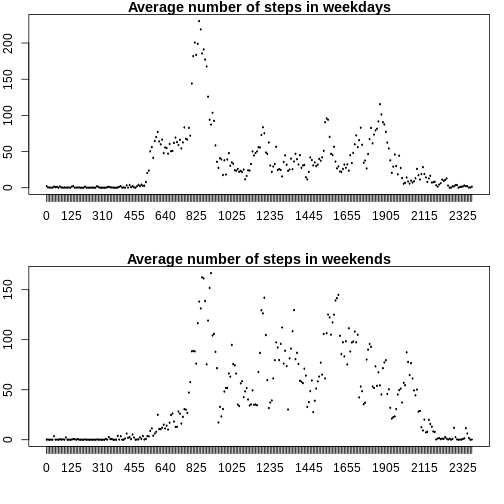
\includegraphics{my_project_files/figure-latex/unnamed-chunk-11-1.pdf}

\end{document}
